%% sudo yum install tetex
%% sudo yum install texlive-elsarticle.noarch  texlive-sttools.noarch texlive-lipsum.noarch
%% pdflatex neural_network.tex && bibtex neural_network.aux && pdflatex neural_network.tex && pdflatex neural_network.tex


%\documentclass[a4paper,12pt]{}
\documentclass[final, paper=letter,5p,times,twocolumn]{elsarticle}
%\documentclass[preprint,review,8pt,times]{elsarticle}


%% or use the graphicx package for more complicated commands
%\usepackage{changebar}
\usepackage{graphicx}
\usepackage{caption}
\usepackage{subcaption}
\usepackage{multirow}
%% or use the epsfig package if you prefer to use the old commands
%% \usepackage{epsfig}

%% The amssymb package provides various useful mathematical symbols
\usepackage{tikz}
\usepackage{amsmath,amsfonts,amsthm,multicol,bm,lipsum} % Math packages
\usepackage{cuted}
%\usepackage{dsfont} % mathds{1}
%\usepackage{widetext} % 
\usepackage{listings}
\usepackage{amssymb}
\usepackage{hyperref}
%
%\usepackage[]{algorithm2e}
%% Macro
\newcommand{\ToDo}[1]{ToDo: \textbf{\textit{#1}}}
\newcommand{\CA}{computational anatomy}
%
\newdefinition{definition}{Definition}%
\newtheorem{theorem}{Theorem}%
\newtheorem{corollary}{Corollary}[theorem]
\newtheorem{lemma}[theorem]{Lemma}
%\newproposition{proposition}{Proposition}%
%\newlemma{lemma}{Lemma}%
%\AtEndEnvironment{theorem}{\null\hfill\qedsymbol}%

\begin{document}
%%%%%%%%%%%%%%%%%%%%%%%%%%%%%%%%%%%%%%%%%%%%%%%%%%%%%%%%%%%%%%%%%%%%%%%%%%
%%%%%%%%%%%%%%%%%%%%%%%%%%%%%%%%%%%%%%%%%%%%%%%%%%%%%%%%%%%%%%%%%%%%%%%%%%
%%%%%%%%%%%%%%%%%%%%%%%%%%%%%%%%%%%%%%%%%%%%%%%%%%%%%%%%%%%%%%%%%%%%%%%%%%
%%%%%%%%%%%%%%%%%%%%%%%%%%%%%%%%%%%%%%%%%%%%%%%%%%%%%%%%%%%%%%%%%%%%%%%%%%
\begin{frontmatter}

\title{Neural network}

\author[label1]{Yann Cobigo\corref{cor1}}
\address[label1]{University of California, San Francisco | ucsf.edu}
%\address[label2]{Address Two\fnref{label4}}

%\cortext[cor1]{I am corresponding author}
%\fntext[label3]{I also want to inform about\ldots}
%\fntext[label4]{Small city}

\ead{yann.cobigo@ucsf.edu}
\ead[url]{https://github.com/YannCobigo}

%% \author[label5]{Author Two}
%% \address[label5]{Some University}
%% \ead{author.two@mail.com}
%% 
%% \author[label1,label5]{Author Three}
%% \ead{author.three@mail.com}

\begin{abstract}
In this report we will \dots
\end{abstract}

\begin{keyword}
%% keywords here, in the form: keyword \sep keyword
Fijee \sep electrode \sep PEM \sep CEM
%% MSC codes here, in the form: \MSC code \sep code
%% or \MSC[2008] code \sep code (2000 is the default)
\end{keyword}

\end{frontmatter}

%%%%%%%%%%%%%%%%%%%%%%%%%%%%%%%%%%%%%%%%%%%%%%%%%%%%%%%%%%%%%%%%%%%%%%%%%%
%%%%%%%%%%%%%%%%%%%%%%%%%%%%%%%%%%%%%%%%%%%%%%%%%%%%%%%%%%%%%%%%%%%%%%%%%%
%%%%%%%%%%%%%%%%%%%%%%%%%%%%%%%%%%%%%%%%%%%%%%%%%%%%%%%%%%%%%%%%%%%%%%%%%%
%%%%%%%%%%%%%%%%%%%%%%%%%%%%%%%%%%%%%%%%%%%%%%%%%%%%%%%%%%%%%%%%%%%%%%%%%%

\section{Introduction}

\paragraph{Inputs}{For the different type of neural networks we would like to accomplish, the input classes must be very differents. Most of the time we are going to work with medical images, implying using a dimensional correlation like the convolutional neural network (CNN). Unlike most of the machine learning algorithm taking vectors as input, CNN void the space decorrelation from the vectorization. However, providing different calsses for different inputs could offer some flexibility.}

\ToDo{check ll sort of input we would want.} \\

%%%%%%%%%%%%%%%%%%%%%%%%%%%%%%%%%%%%%%%%%%%%%%%%%%%%%%%%%%%%%%%%%%%%%%%%%%
%%%%%%%%%%%%%%%%%%%%%%%%%%%%%%%%%%%%%%%%%%%%%%%%%%%%%%%%%%%%%%%%%%%%%%%%%%
\section{Functions}

A neuron is represented with an activation $a_{l_{i}} = \sum_{l_{j} = 0}^{L_{j}} \omega_{l_{i}l_{j}} z_{l_{j}}$, integrating pulses from other neurons, and its activation function $z_{l_{i}} = f(a_{l_{i}})$, the firering process of the neuron. Usually, the activation function is taken non-linear. Following the litterature, we will mostly use $\tanh$ or logistic function.

\subsection{Activation functions}

\subsubsection{Soft maximum}
\label{soft_max_sec}

The soft maximum is often used in classfication problem involving multiple output classes. the output can be interpretated as probability following the distribution:

\begin{equation}
  g(a_{l_{k}}) = \frac{e^{a_{l_{k}}}}{\mathcal{Z}}
  \label{soft_max}
\end{equation}

Where $\mathcal{Z}$ is the partition function normalizing the distribution. Derivating the soft maximum in function of the parameter $a_{k}$ gives us:

\begin{equation*}
  \begin{split}
    \frac{\partial g(a_{k})}{\partial a_{k'}} = & \left \lbrack \delta_{kk'} e^{a_{k'}} \mathcal{Z} - e^{a_{k'}}\frac{\partial \mathcal{Z}}{\partial a_{k'}} \right \rbrack \times \frac{1}{\mathcal{Z}^{2}}\\
    = & \left \lbrack \delta_{kk'} e^{a_{k'}} \mathcal{Z} - e^{a_{k'}} \sum_{k''} \delta_{kk''} e^{a_{k''}}  \right \rbrack \times \frac{1}{\mathcal{Z}^{2}}\\
    = & \frac{\delta_{kk'} e^{a_{k'}}}{\mathcal{Z}} - z_{k}z_{k'}\\
  \end{split}
\end{equation*}


\subsection{Cost functions}

Training the neural network uses the gradient method. All functions representing the neural activity needs to be differentiable, including the cost fuction.

\subsubsection{Least-squarre cost function}

\begin{equation}
  E = \frac{1}{2} \sum_{i = 1}^{n} \| \bm{z}(\bm{x}_{i}) - \bm{t}_{i} \|^{2}
  \label{least_squarre}
\end{equation}

\subsubsection{Cross entropy cost function}
\label{Cross_entropy_cost_function_sec}

In information theory, the cross entropy between two probability distributions $p$ and $q$ over the same underlying set of events measures the average number of bits needed to identify an event drawn from the set, if a coding scheme is used that is optimized for an "unnatural" probability distribution $q$, rather than the "true" distribution $p$. In classification, the cross entropy for the distributions $t$, labels, and $z$, reconstructed solution, over a given set is defined as follows:

\begin{equation}
  E = - \sum_{i = 1}^{n}\sum_{l'_{k} = 1}^{L_{k}} t_{l'_{k}} \ln z_{l'_{k}} =  - \sum_{i = 1}^{n} E_{i}
  \label{cross_entropy}
\end{equation}

$t_{l'_{k}}$ represents the known label, $z_{l'_{k}} = y_{k}$ represents the response of the system, $n$ is the number of participents. 

In this section, we are going to derivate the cross entropy~(\ref{cross_entropy}). To simplify the equation, we are derivating the cost function only for one subject and omitte the subscript $i$. At the output layer, the activation is $a_{l_{k}} = \sum_{l_{k-1} = 0}^{L_{k-1}} \omega_{l_{k}l_{k-1}} z_{l_{k-1}}$. The derivative of the cost function in function of the activtion is called the {\it error} and is written:

\begin{equation}
  \delta_{k} = \frac{\partial E}{\partial a_{l_{k}}} = - \sum_{l'_{k} = 1}^{L_{k}} t_{l'_{k}} \times \frac{1}{z_{l'_{k}}} \frac{\partial z_{l'_{k}}}{\partial a_{k}}
  \label{cost_function_error}
\end{equation}

In the case of the last activation fuction for the output layer is a soft maximum, we can use the result of the soft maximum derivative from the paragraph~\ref{soft_max_sec}:

\begin{equation*}
  \begin{split}
    \delta_{k} = & - \sum_{l'_{k} = 1}^{L_{k}} t_{l'_{k}} \times \frac{1}{z_{l'_{k}}} \left \lbrack  \frac{\delta_{kk'} e^{a_{l'_{k}}}}{\mathcal{Z}} - z_{l'_{k}}z_{l_{k}} \right \rbrack \\
    = & - \sum_{l'_{k} = 1}^{L_{k}} t_{l'_{k}} \times \frac{1}{z_{l'_{k}}} \frac{\delta_{kk'} e^{a_{l'_{k}}}}{\mathcal{Z}} +  \sum_{l'_{k} = 1}^{L_{k}} t_{l'_{k}} z_{l_{k}} \\
    = & - t_{l_{k}} +  z_{k} \\
  \end{split}
\end{equation*}



Which is exactly the same result as we would get in the cas of a least-square cost function.


%%%%%%%%%%%%%%%%%%%%%%%%%%%%%%%%%%%%%%%%%%%%%%%%%%%%%%%%%%%%%%%%%%%%%%%%%%
%%%%%%%%%%%%%%%%%%%%%%%%%%%%%%%%%%%%%%%%%%%%%%%%%%%%%%%%%%%%%%%%%%%%%%%%%%
\section{Convolutional neural network}

Convolutional neural networks (CNNs) are a biologically-inspired variation of the multilayer perceptrons (MLPs). Neurons in CNNs share weights unlike in MLPs where each neuron has a separate weight vector. This sharing of weights ends up reducing the overall number of trainable weights hence introducing sparsity. The output image is downsampled to reduce the number of weights for the next neural network and prevent overfitting.

\subsection{Description and notation}

CNNs consists of convolutional layers which are characterized by an input map $Im$, a bank of filters $Ker$ and biases $b$ per layer. Utilizing the weights sharing strategy, each neuron in the feature map is the result of the convolution of a kernel with a region in the input image, called the {\it local receptive field for the hidden neuron}, Fig.~\ref{fig:Convolutional_layers}. The local receptive field is a little window on the input pixels. You can think of that particular hidden neuron as learning to analyze its particular local receptive field. This is then followed by a pooling operation which as a form of non-linear down-sampling, progressively reduces the spatial size of the representation thus reducing the amount of computation and parameters in the network. Existing between the convolution and the pooling layer is an activation function such as the Rectified Linear unit ({\it ReLu}) layer; a non-saturating activation is applied element-wise, {\it i.e.} $f(x) = \max(0,x)$ thresholding at zero. After several convolutional and pooling layers, the image size (feature map size) is reduced and more complex features are extracted. \\
Eventually with a small enough feature map, the contents are squashed into a one dimension vector and fed into a fully-connected MLP for processing. The last layer of this fully-connected MLP seen as the output, is a loss layer which is used to specify how the network training penalizes the deviation between the predicted and true labels.


\begin{figure}[htbp]
   \begin{center}
      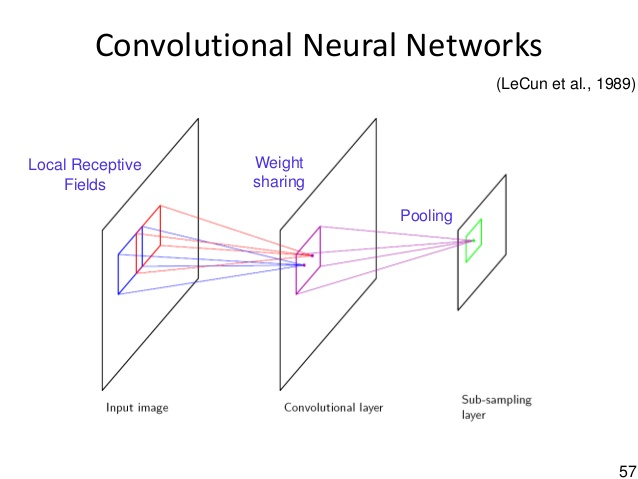
\includegraphics[scale=0.3, angle=0]{images/Bishop_cnn_layer.jpg}
   \end{center}
   \caption{Convolutional layers.}
  \label{fig:Convolutional_layers} 
\end{figure}

\begin{figure*}[htbp]
   \begin{center}
      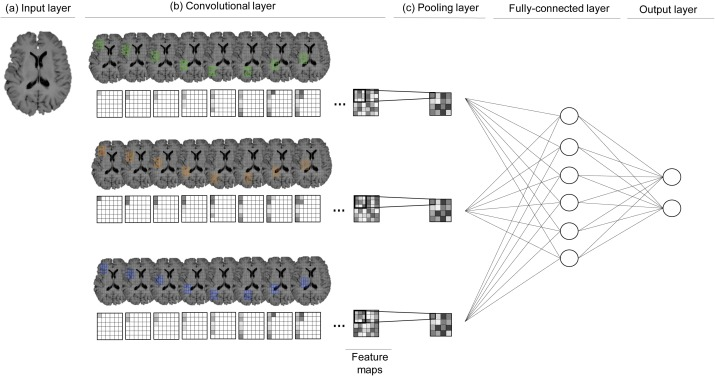
\includegraphics[scale=1., angle=0]{images/1-s2_0-S0149763416305176-gr4.jpg}
   \end{center}
   \caption{Generic structure of a CNN. For illustrative purpose, this example only has one layer of each type; a real-world CNN, however, would have several convolutional and pooling layers (usually interpolated) and one fully-connected layer. (a) Input layer. In its simplest way, the data is inputted into the network in such a way that each pixel corresponds to one node in the input layer. (b) Convolutional layer. A $3 \times 3$ filter or kernel (in green) is used to multiply the spatially corresponding $3 \times 3$ nodes in the image. The resulting weighted sum is then passed through a nonlinear function to derive the output value of one node in the feature map. The repetition of this same operation across all possible receptive fields results in one complete feature map. The same procedure with different kernels (in orange and blue) will result in separate complete feature maps. (c) Pooling layer. The size of each feature map can be reduced by taking the maximum value (or average) from a receptive field in the previous layer. (For interpretation of the references to colour in this figure legend, the reader is referred to the web version of this article.)}
  \label{fig:features_maps} 
\end{figure*}

\paragraph{Feature map}{The weights sharing strategy means that all the neurons in the first hidden layer detect exactly the same feature at different locations in the input image. A feature detected by a hidden neuron as the kind of input pattern that will cause the neuron to activate: it might be an edge in the image, for instance, or maybe some other type of shape. To see why this makes sense, suppose the weights and bias are such that the hidden neuron can pick out, a vertical edge in a particular local receptive field. That ability is also likely to be useful at other places in the image. And so it is useful to apply the same feature detector everywhere in the image. To put it in slightly more abstract terms, convolutional networks are well adapted to the translation invariance of images: move a picture of a cat a little ways, and it's still an image of a cat. To increase the feature coverage we create multiple kernel and use the same procedure with different kernels (in orange and blue) will result in separate complete feature maps Fig.~\ref{fig:features_maps} (\ToDo{How to initial the weights between two feature maps?})}

\subsubsection{Convolution}

Given a three dimentional input image $Im$ and a filter (kernel) $Ker$ of dimensions $I \times J \times K$, the convolution operation is given by:

\begin{equation}
  \begin{split}
    (Im*Ker)_{xyz} = & \sum_{i=1}^{I}\sum_{j=1}^{J}\sum_{k=1}^{K}Im(x-i,y-j,z-k)Ker(i,j,k)\\
    = & \sum_{i=1}^{I}\sum_{j=1}^{J}\sum_{k=1}^{K}Im(x+i,y+j,z+k)Ker(-i,-j,-k)
  \end{split}
  \label{eq:convolution} 
\end{equation}

Eq.~(\ref{eq:convolution}) is represented on the Fig~\ref{fig:Kernel}. In the case of neuroimages, we could have $M$ modalities as inputs such that $Im \in \mathbb{R}^{X \times Y \times Z}$. Subsequently, for one convolutional layer with a bank of $D$ filters we have $Ker \in \mathbb{R}^{I \times J \times K \times D}$ and biases $b \in \mathbb{R}^{D}$, one for each filter. The feature map is for a modality $m$:

\begin{equation*}
    (Im*Ker)_{x,y,z,m} =  \sum_{i=1}^{I}\sum_{j=1}^{J}\sum_{k=1}^{K}Im_{x+i,y+j,z+k,m}Ker_{-i,-j,-k,-m} - b_{x,y,z,m}
  \label{eq:convolution_tot} 
\end{equation*}

For a layer's voxel:

\begin{equation}
    a_{xyz;l_{u}}^{(\theta)} =  \sum_{i=1,j=1,k=1}^{I \times J \times K}\omega_{ijk;l_{u}}^{(\theta)}z_{x+i,y+j,z+k;l_{u-1}}^{(\theta)} - b_{l_{k}}^{(\theta)}
  \label{eq:convolution_tot_vox} 
\end{equation}

where $a$ is the convolved activation voxel in the feature map, $l_{u}$ is any layer, $\omega$ is the weight at the layer $l_{u}$ (Fig.~\ref{fig:Kernel}), $b$ is the bias at the level $l_{u}$, $z$ is the output at the level $l_{u-1}$ ($z_{xyz;l_{u}}^{(\theta)} = f(a_{xyz;l_{u}}^{(\theta)})$ where $f$ is an activation function). $\theta = \{m,d\}$ is the set of parameters describing the modality $m$ and the set of kernels $d$ associated to the different feature maps.



\begin{figure}[htbp]
   \begin{center}
      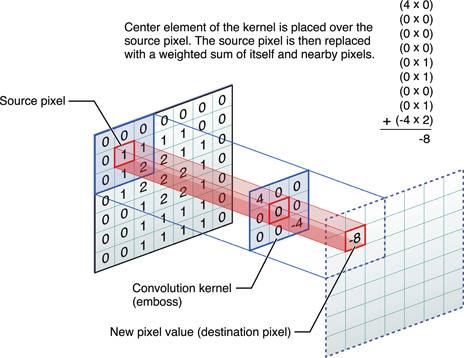
\includegraphics[scale=0.3, angle=0]{images/GvsBA.jpg}
   \end{center}
   \caption{Kernel. Two dimensions representation of the kernel action.}
  \label{fig:Kernel} 
\end{figure}



\subsection{Foward Propagation}

To perform a convolution operation, the kernel is flipped $180^{\circ}$ and slid across the input feature map in equal and finite strides. At each location, the product between each element of the kernel and the input feature map element it overlaps is computed and the results summed up to obtain the output at that current location Fig.~\ref{fig:Kernel} modelized by Eq.~(\ref{eq:convolution_tot_vox}). This procedure is repeated using different kernels to form as many output feature maps as desired Fig.~\ref{fig:features_maps}. The concept of weight sharing is used as demonstrated in the diagram Fig.~\ref{fig:fCNN}.

\begin{figure}[htbp]
   \begin{center}
      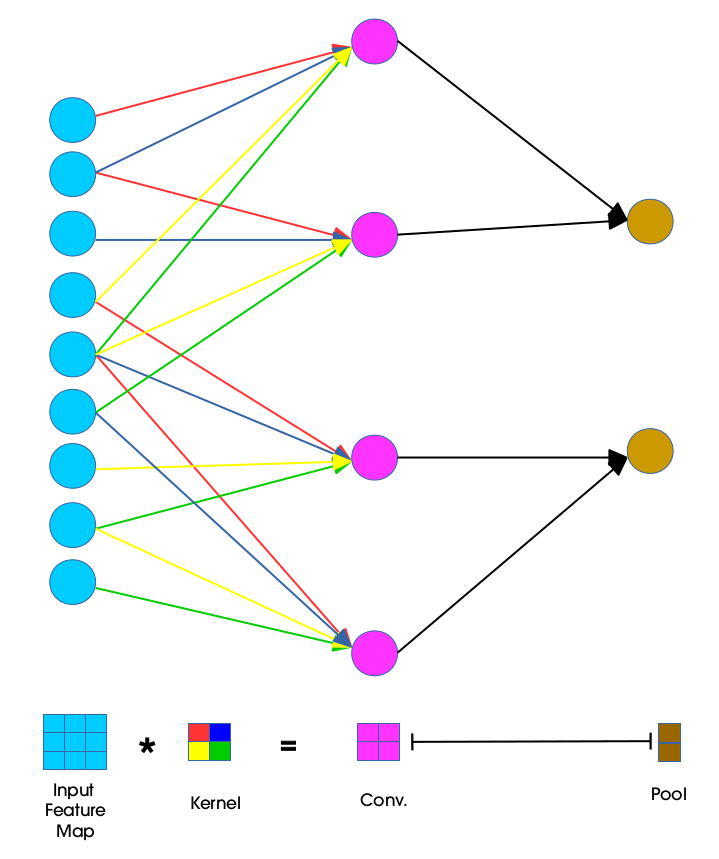
\includegraphics[scale=0.3, angle=0]{images/fCNN.png}
   \end{center}
   \caption{Units in convolutional layer illustrated above have receptive fields of size 4 in the input feature map and are thus only connected to 4 adjacent neurons in the input layer. This is the idea of sparse connectivity in CNNs where there exists local connectivity pattern between neurons in adjacent layers.}
  \label{fig:fCNN} 
\end{figure}

\subsection{Backpropagation}

For backpropagation there are two updates performed, for the weights and the deltas. Lets begin with the weight update. We are looking to compute $\partial E / \partial \omega_{uvw;l}^{(\theta)}$ which can be interpreted as the measurement of how the change in a single pixel $\omega_{uvw;l}^{(\theta)}$ in the weight kernel affects the loss function $E$. Convolution between the input feature map of dimension $X \times Y \times Z$  and the weight kernel of dimension $I \times J \times K$ produces an output feature map of size $X \times Y \times Z$. The gradient component for the individual weights can be obtained by applying the chain rule Eq.~(\ref{eq:conv_backward_weights}).\\

%\lipsum[3-4]

\begin{equation}
  \begin{split}
    \frac{\partial E_{i}}{\partial \omega_{uvw;l_{u}}^{(\theta)}} =& \sum_{xyz}^{X \times Y \times Z} \frac{\partial E_{i}}{\partial a_{xyz;l_{u}}^{(\theta)}}\frac{\partial a_{xyz;l_{u}}^{(\theta)}}{\partial \omega_{uvw;l_{u}}^{(\theta)}}  \\
    =& \sum_{xyz}^{X \times Y \times Z} \delta_{l_{u}}^{(\theta)}z_{x'+u,y'+v,z'+w;l_{u-1}}^{(\theta)} \\
  \end{split}
  \label{eq:conv_backward_weights} 
\end{equation}

Using equation~(\ref{eq:convolution_tot_vox}) for all the activation of the layer $l_{u}$, we have:

\begin{equation*}
    \left( \frac{\partial a_{xyz;l_{u}}}{\partial \omega_{uvw;l_{u}}} \right)^{(\theta)} = z_{x'+u,y'+v,z'+w;l_{u-1}}^{(\theta)}
\end{equation*}

Where $(x',y',z')$ are in the receiptive field of $(x,y,z)$. In our case, the input map and the feature map have exactly the the size, we should have a strict correspondance between $(x',y',z')_{l_{k}}$ and $(x,y,z)_{l_{k-1}}$. The second part of the equation can be solved in the following way:


\begin{strip}
\begin{equation}
  \begin{split}
    \frac{\partial E_{i}}{\partial a_{xyz;l_{u}}^{(\theta)}} =&  \sum_{x''y''z''}^{X \times Y \times Z} \frac{\partial E_{i}}{\partial a_{x''y''z'';l_{u+1}}^{(\theta'')}}\frac{\partial a_{x''y''z'';l_{u+1}}^{(\theta'')}}{\partial a_{xyz;l_{u}}^{(\theta)}}\\
    =& \sum_{x''y''z''}^{X \times Y \times Z} \delta_{l_{u+1}}^{(\theta'')}(x'',y'',z'') \times \frac{\partial a_{x''y''z'';l_{u+1}}^{(\theta'')}}{\partial a_{xyz;l_{u}}^{(\theta)}}\\
    =& \sum_{x''y''z''}^{X \times Y \times Z} \delta_{l_{u+1}}^{(\theta'')}(x'',y'',z'') \times \frac{\partial }{\partial a_{xyz;l_{u}}^{(\theta)}} \sum_{abc}\omega_{abc;l_{u+1}}^{(\theta)}f(a_{x''+a,y''+b,z''+c;l_{u}}^{(\theta)})\\
    =& \sum_{x''y''z''}^{X \times Y \times Z} \delta_{l_{u+1}}^{(\theta'')}(x'',y'',z'') \times \sum_{abc}\omega_{abc;l_{u+1}}^{(\theta'')} \delta(x-(x''+a),y-(y''+b),z-(z''+c)) f'(a_{x''+a,y''+b,z''+c;l_{u}}^{(\theta)})\\
    =& f'(a_{x,y,z;l_{u}}^{(\theta)}) \sum_{abc} \delta_{l_{u+1}}^{(\theta'')}(x-a,y-b,z-c) \times \omega_{abc;l_{u+1}}^{(\theta'')} \\
  \end{split}
  \label{} 
\end{equation}
\end{strip}

Where $\{(x'',y'',z'')_{l_{k}}\}$ is a set of activation sites on the layer $l_{u+1}$ having $(x,y,z)_{l_{k}}$ in its receiving field. We keep the $\delta(x-(\tilde{x}+a),y-(\tilde{y}+b),z-(\tilde{z}+c))$ Dirac distribution in the sum, since we will select the $(a,b,c)$ to get an input output correspondance. 

\subsection{Pooling Layer}

The function of the pooling layer is to progressively reduce the spatial size of the representation to reduce the amount of parameters and computation in the network, and hence to also control overfitting. No learning takes place on the pooling layers. Pooling units are obtained using functions like max-pooling, average pooling and even L2-norm pooling. At the pooling layer, forward propagation results in an $N \times N$ pooling block being reduced to a single value -- value of the {\it winning unit}. Backpropagation of the pooling layer then computes the error which is acquired by this single value winning unit. To keep track of the winning unit its index noted during the forward pass and used for gradient routing during backpropagation. Gradient routing is done in the following ways:

\begin{itemize}
    \item Max-pooling - the error is just assigned to where it comes from - the “winning unit” because other units in the previous layer’s pooling blocks did not contribute to it hence all the other assigned values of zero
    \item Average pooling - the error is multiplied by $1 / (N \times N)$ and assigned to the whole pooling block (all units get this same value).
\end{itemize}

%%%%%%%%%%%%%%%%%%%%%%%%%%%%%%%%%%%%%%%%%%%%%%%%%%%%%%%%%%%%%%%%%%%%%%%%%%
%%%%%%%%%%%%%%%%%%%%%%%%%%%%%%%%%%%%%%%%%%%%%%%%%%%%%%%%%%%%%%%%%%%%%%%%%%
\section{Densely connected neural network}
\subsection{Description and notation}

Dense neural networks are cracterized by a full connection of a neuron of one layer with all neurons from the previouse layer. Table~\ref{Layers_activations} presents the activation function for each layer. In this document, the convention is $l = l_{0}$ for the input layer: $z_{l_{0} = 1} = x_{1}$, $z_{l_{0} = 2} = x_{2}$, \dots We will reserve the index 0 for the bias: $z_{l_{0} = 0} = x_{0} = b_{0}$ the bias on the input level. The last level is the output level: $l = l_{k}$, $z_{l_{k}} = y_{k}$. The output level does not have a bias node.

\begin{table}[]
\centering
\caption{Neuron activation for each layers.}
\label{Layers_activations}
\begin{tabular}{llllll}
 $\{ z_{l_{0}}\}_{l_{0} = 0}^{L_{0}}$&  $\{ z_{l_{1}}\}_{l_{1} = 0}^{L_{1}}$ &  $\cdots$ & $\{ z_{l_{k-1}}\}_{l_{k-1} = 0}^{L_{k-1}}$ &  $\{ z_{l_{k}}\}_{l_{k} = 1}^{L_{k}}$ &  \\ 
\end{tabular}
\end{table}

\begin{figure}[htbp]
   \begin{center}
      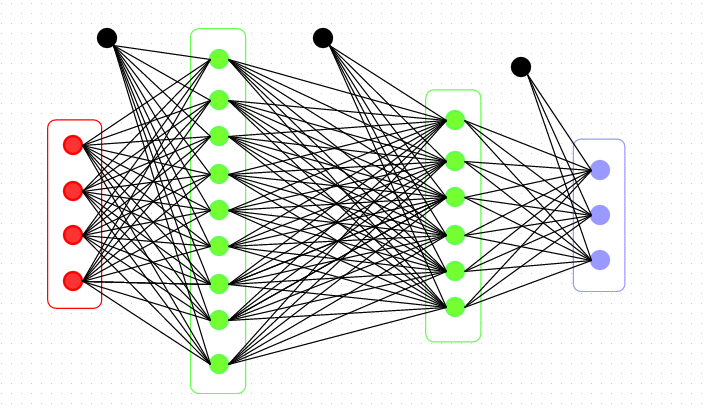
\includegraphics[scale=0.3, angle=0]{images/densely_connected_nn.png}
   \end{center}
   \caption{Densely connected neural network.}
  \label{fig:Densely_connected_neural_network} 
\end{figure}




Each neuron is an activated function, $f$, of a linear combinaison of the neurons from the previous layer. Function $g$ is the activation function for the output layer.

\begin{itemize}
    \item $l = l_{0}$ we are at the level of the inputs
    \item $l = l_{1}$ $a_{l_{1}} = \sum_{l'_{0} = 0}^{L_{0}} \omega_{l_{1}l'_{0}} z_{l'_{0}} = \omega_{l_{1}}^{T} z^{(0)}$. \\ And $z_{l_{1}} = f(a_{l_{1}})$ \\
     $\vdots$
    \item $l = l_{k-1}$ $a_{l_{k-1}} = \sum_{l'_{k-2} = 0}^{L_{k-2}} \omega_{l_{k-1}l'_{k-2}} z_{l'_{k-2}} = \omega_{l_{k-1}}^{T} z^{(k-2)}$. \\ And $z_{l_{k-1}} = f(a_{l_{k-1}})$
    \item $l = l_{k}$ $a_{l_{k}} = \sum_{l'_{k-1} = 0}^{L_{k-1}} \omega_{l_{k}l'_{k-1}} z_{l'_{k-1}} = \omega_{l_{k}}^{T} z^{(k-1)}$. \\ And $z_{l_{k}} = g(a_{l_{k}})$
\end{itemize}

In this enumeration $z^{(i)}$ is a vector of all neurons on the layer $(i)$. There are several choises for the activation function and we will try to provide the possibility of using several of them. However, the first developpments will be done with the hyperbolic tangent for the activation of the inside layers neurons: $f = \tanh$ and $f' = (1 - \tanh^{2})$. The last layer, the output layer, will be calculated with a soft maximum: $g(z_{l_{k}}) = e^{a_{l_{k}}} / \mathcal{Z}$, where the partition function $\mathcal{Z} = \sum_{l_{k} = 1}^{L_{k}} e^{z_{l_{k}}}$, and $g' = g(1 - g)$.
  
\subsection{Forward propagation}

The forward propagation is straight forward. For a solution, $y_{k} = z_{l_{k}} = g(a_{l_{k}})$ where
$$
a_{l_{k}} = \omega_{l_{k}}^{T} z^{(k-1)} = \omega_{l_{k}}^{T} f(\omega_{l_{k-1}}^{T} z^{(k-2)}) = \omega_{l_{k}}^{T} f(\omega_{l_{k-1}}^{T} f(\omega_{l_{k-2}}^{T} z^{(k-3)})) = \dots
$$

\subsubsection{Algorithm}

The Table~\ref{weights_distribution} gives the distribution of the weights in a dense neural network. These weights can be represented in one long array in the hardware memory, Table~\ref{weights_in_mem}. The first layer $l = l_{1}$, after the inputs, has $(L_{1}-1)\times(L_{0})$ weights. The layer after has $(L_{2}-1)\times(L_{1})$ weights, so forth till the last layer having $L_{k}\times(L_{k-1})$.

\begin{table}[]
\centering
\caption{Weight distribution per layer.}
\label{weights_distribution}
\begin{tabular}{|c|c|c|c|c|c|}
\hline
$l_{0}$                   && 0                                   & 1                        & $\cdots$ & $L_{0}$ \\ \hline
\multirow{4}{*}{$l_{1}$}  &0& $\omega_{l_{1}=0l_{0}=0}$              & $\omega_{l_{1}=0l_{0}=1}$    &        & $\omega_{l_{1}=0l_{0}=L_{0}}$ \\ \cline{2-6} 
                         &1& $\omega_{l_{1}=1l_{0}=0}$              & $\omega_{l_{1}=1l_{0}=1}$    &        & $\omega_{l_{1}=0l_{0}=L_{0}}$ \\ \cline{2-6} 
                         &&                                     &                          & \vdots & \\ \cline{2-6} 
                         &$L_{1}$& $\omega_{l_{1}=L_{1}l_{0}=0}$      & $\omega_{l_{1}=L_{1}l_{0}=1}$ &        & $\omega_{l_{1}=L_{1}l_{0}=L_{0}}$ \\ \hline
$l_{1}$                   && 0                                   & 1                       &        & $L_{1}$ \\ \hline
\multirow{4}{*}{$l_{2}$}  &0& $\omega_{l_{2}=0l_{1}=0}$              &  $\omega_{l_{2}=0l_{1}=1}$   &        &  $\omega_{l_{2}=0l_{1}=L_{1}}$ \\ \cline{2-6} 
                         &1& $\omega_{l_{2}=1l_{1}=0}$              &  $\omega_{l_{2}=1l_{1}=1}$   &        &   $\omega_{l_{2}=0l_{1}=L_{1}}$ \\ \cline{2-6} 
                         &&                                     &                          & \vdots & \\ \cline{2-6} 
                         &$L_{2}$&$\omega_{l_{2}=L_{2}l_{1}=0}$       & $\omega_{l_{2}=L_{2}l_{1}=1}$ &        & $\omega_{l_{2}=L_{2}l_{1}=L_{1}}$ \\ \hline
\vdots                   &&                                     &                         &        & \\ \hline
$l_{k-1}$                 && 0                                   &  1                      &        &  $L_{k-1}$ \\ \hline
\multirow{4}{*}{$l_{k}$}  &1& $\omega_{l_{k}=1l_{k-1}=0}$            & $\omega_{l_{k}=1l_{k-1}=1}$  &        & $\omega_{l_{k}=1l_{k-1}=L_{k-1}}$ \\ \cline{2-6} 
                         &2& $\omega_{l_{k}=2l_{k-1}=0}$            & $\omega_{l_{k}=2l_{k-1}=1}$  &        &  $\omega_{l_{k}=2l_{k-1}=L_{k-1}}$ \\ \cline{2-6} 
                         &&                                    &                         & \vdots & \\ \cline{2-6} 
                         &$L_{k}$& $\omega_{l_{k}=L_{k1}l_{k-1}=0}$   & $\omega_{l_{k}=L_{k}l_{k-1}=1}$ &        &  $\omega_{l_{k}=L_{k}l_{k-1}=L_{k-1}}$ \\ \hline
\end{tabular}
\end{table}

\begin{table}[]
\centering
\caption{Representation in a one dimension array of the all the weights.}
\label{weights_in_mem}
\begin{tabular}{|c|c|c|c|c|c|c|c|}
\hline
\multicolumn{4}{|c|}{$l_{1}$} & $\hdots$ & \multicolumn{3}{c|}{$l_{k}$} \\ \hline
$\omega_{l_{1}=0l_{0}=0}$   &   $\omega_{01}$   & $\hdots$  &  $\omega_{L_{1}L_{0}}$   & $\hdots$ &    $\omega_{l_{k}=1l_{k-1}=0}$    & $\hdots$  &   $\omega_{L_{k}L_{k-1}}$ \\ \hline
\end{tabular}
\end{table}

%%%%%%%%%%%%%%%%%%%%%%%%%%%%%%%%%%%%%%%%%%%%%%%%%%%%%%%%%%%%%%%%%%%%%%%%%%
%%%%%%%%%%%%%%%%%%%%%%%%%%%%%%%%%%%%%%%%%%%%%%%%%%%%%%%%%%%%%%%%%%%%%%%%%%
\subsection{Backward propagation}

To solve the problem of the backward propagation, we have three options. The first option is to estimate the error for the full training set, which is heavy for the algorithm. The second option is the gradient descent in its stochastic version: each iteration will use a new intput, instead of estimating the cost function with the entire input population. The third option is a mid point between the two first option: the error is estimated with a batches sub set of the full training set.
Taking the cross-enropy cost function, eq.~(\ref{cross_entropy}), in the case of classificaion. The gradient descent method used to find the minimum of the cost function is written:

\begin{equation}
  \bm{\omega}^{e+1} = \bm{\omega}^{e} - \eta \bm{\nabla} E
  \label{gradient_descent}
\end{equation}

Where $\bm{\omega}$ represents the vector of weights, $e$ represents the {\it epoque}, and $\eta$ represents the learning rate. 


%%%%%%%%%%%%%%%%%%%%%%%%%%%%%%%%%%%%%%%%%%%%%%%%%%%%%%%%%%%%%%%%%%%%%%%%%%
\subsubsection{Algorithm}

The backward propagation for each layer, except the last layer, is a recursive estimtion of the deeper layer. The gradient~(\ref{gradient_descent}) at a particular weight is

\begin{equation*}
  \frac{\partial E_{i}}{\partial \omega_{l_{u}l_{v}}} = \frac{\partial E_{i}}{\partial a_{l_{u}}} \frac{\partial a_{l_{u}}}{\partial \omega_{l_{u}l_{v}}} = \delta_{l_{u}}\frac{\partial a_{l_{u}}}{\partial \omega_{l_{u}l_{v}}} 
\end{equation*}


\paragraph{$\bm{l = l_{k}}$}{ Using the results from the section~\ref{Cross_entropy_cost_function_sec}:

  \begin{equation*}
    \begin{split}
      \frac{\partial E_{i}}{\partial \omega_{l_{k}l_{k-1}}} = &  \frac{\partial E_{i}}{\partial a_{l_{k}}} \frac{\partial a_{l_{k}}}{\partial \omega_{l_{k}l_{k-1}}}  \\
              = &  (z_{l_{k}} - t_{l_{k}})z_{l_{k-1}} \\
    \end{split}
  \end{equation*}

}

\paragraph{$\bm{l = l_{u}}$}{We write the relation between the level $l_{u}$ and the layer immediatly after using the chain rules of partial derivative:

  \begin{equation*}
    \begin{split}
      \frac{\partial E_{i}}{\partial \omega_{l_{u}l_{u-1}}} = &  \frac{\partial E_{i}}{\partial a_{l_{u}}} \frac{\partial a_{l_{u}}}{\partial \omega_{l_{u}l_{u-1}}} = \delta_{l_{u}} \frac{\partial a_{l_{u}}}{\partial \omega_{l_{u}l_{u-1}}}  \\
              = & \sum_{l'_{u+1}}\frac{\partial E_{i}}{\partial a_{l'_{u+1}}} \frac{\partial a_{l'_{u+1}}}{\partial a_{l_{u}}} \frac{\partial a_{l_{u}}}{\partial \omega_{l_{u}l_{u-1}}}   \\
              = & \sum_{l'_{u+1}} \delta_{l'_{u+1}} \frac{\partial a_{l'_{u+1}}}{\partial a_{l_{u}}} z_{l_{u-1}}   \\
              = & \sum_{l'_{u+1}} \delta_{l'_{u+1}} \sum_{l'_{u}} \omega_{l'_{u+1}l'_{u}} f'(a_{l'_{u}}) \delta_{l'_{u}l_{u}} z_{l_{u-1}}   \\
              = & \sum_{l'_{u+1}} \delta_{l'_{u+1}} \omega_{l'_{u+1}l_{u}} f'(a_{l_{u}}) z_{l_{u-1}}   \\
    \end{split}
\end{equation*}

}


%%%%%%%%%%%%%%%%%%%%%%%%%%%%%%%%%%%%%%%%%%%%%%%%%%%%%%%%%%%%%%%%%%%%%%%%%%
%%%%%%%%%%%%%%%%%%%%%%%%%%%%%%%%%%%%%%%%%%%%%%%%%%%%%%%%%%%%%%%%%%%%%%%%%%
\section{sect}

%%%%%%%%%%%%%%%%%%%%%%%%%%%%%%%%%%%%%%%%%%%%%%%%%%%%%%%%%%%%%%%%%%%%%%%%%%
%%%%%%%%%%%%%%%%%%%%%%%%%%%%%%%%%%%%%%%%%%%%%%%%%%%%%%%%%%%%%%%%%%%%%%%%%%
\section{sect}

%%%%%%%%%%%%%%%%%%%%%%%%%%%%%%%%%%%%%%%%%%%%%%%%%%%%%%%%%%%%%%%%%%%%%%%%%%
%%%%%%%%%%%%%%%%%%%%%%%%%%%%%%%%%%%%%%%%%%%%%%%%%%%%%%%%%%%%%%%%%%%%%%%%%%
\section{sect}


%%%%%%%%%%%%%%%%%%%%%%%%%%%%%%%%%%%%%%%%%%%%%%%%%%%%%%%%%%%%%%%%%%%%%%%%%%
\section{Conclusion}

\section*{References}
%% References with bibTeX database:
\bibliographystyle{Bibliography/elsarticle-num}

\bibliography{Bibliography/sample}


\end{document}
